\documentclass[11pt,a4paper,landscape]{article}
\usepackage[utf8]{inputenc}
\usepackage[T1]{fontenc}
\usepackage[margin=12mm]{geometry}
\usepackage{tikz}
\usetikzlibrary{arrows.meta,calc,shapes.multipart}
\pagestyle{empty}
\setlength{\parindent}{0pt}

\definecolor{tinta}{HTML}{17364A}
\definecolor{fondo}{HTML}{E9F0F5}
\definecolor{borde}{HTML}{2D5169}

\tikzset{
  clase/.style={
    rectangle split, rectangle split parts=2, rounded corners=1pt,
    draw=borde, line width=.65pt, fill=white,
    rectangle split part fill={fondo,white}, text=tinta,
    text width=4.22cm, inner sep=5pt, align=left
  },
  depende/.style={dashed, draw=borde, -{Stealth[length=2.5mm]}},
  hereda/.style={draw=borde, -{Triangle[open,length=3mm,width=2.8mm]}},
  compone/.style={draw=borde, {Diamond[length=3mm,width=2.1mm]}-},
  etiqueta/.style={fill=white, text=tinta, inner sep=2pt, font=\small}
}

\newcommand{\clase}[4]{%
  \node[clase] (#1) at (#2) {%
    \textbf{\texttt{#3}}\nodepart{second}\small #4%
  };%
}
\newcommand{\titulo}[2]{%
  {\Large\bfseries\color{tinta} #1}\par\smallskip
  {\color{tinta}#2}\par\medskip
}

\begin{document}

\titulo{Veterinaria 2D · MVC y transiciones}
  {Contratos declarados para la clínica, la misión y la interfaz}

\centering
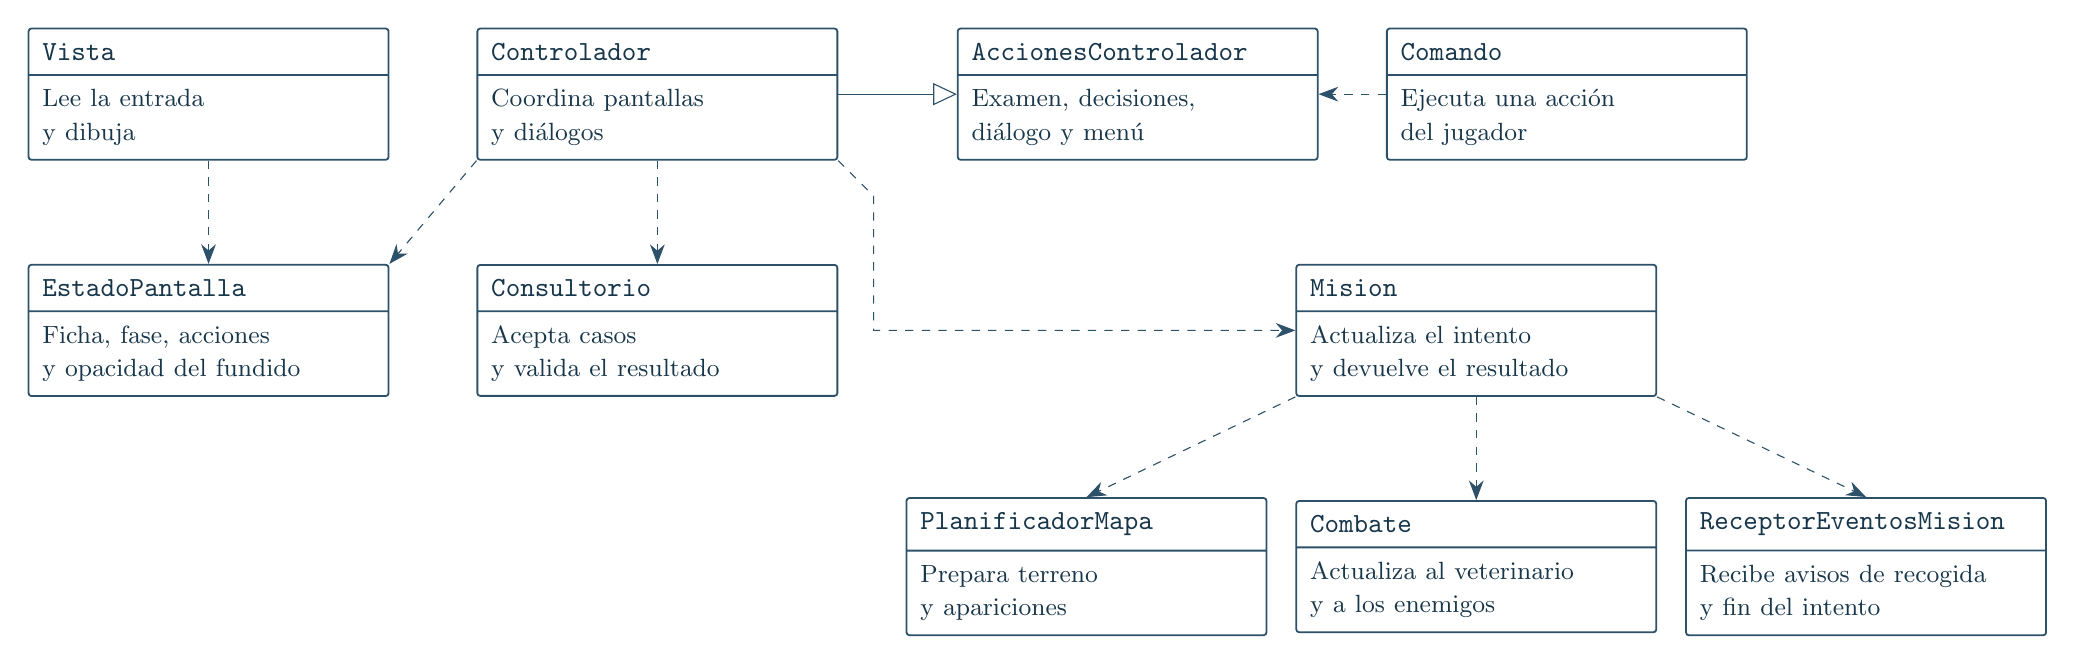
\begin{tikzpicture}
  \clase{vista}{2.4,9.3}{Vista}{Lee la entrada\\y dibuja}
  \clase{controlador}{8.1,9.3}{Controlador}{Coordina pantallas\\y diálogos}
  \clase{acciones}{14.2,9.3}{AccionesControlador}{Examen, decisiones,\\diálogo y menú}
  \clase{comando}{19.65,9.3}{Comando}{Ejecuta una acción\\del jugador}
  \clase{pantalla}{2.4,6.3}{EstadoPantalla}{Ficha, fase, acciones\\y opacidad del fundido}
  \clase{consultorio}{8.1,6.3}{Consultorio}{Acepta casos\\y valida el resultado}
  \clase{mision}{18.5,6.3}{Mision}{Actualiza el intento\\y devuelve el resultado}
  \clase{mapa}{13.55,3.3}{PlanificadorMapa}{Prepara terreno\\y apariciones}
  \clase{combate}{18.5,3.3}{Combate}{Actualiza al veterinario\\y a los enemigos}
  \clase{receptor}{23.45,3.3}{ReceptorEventosMision}{Recibe avisos de recogida\\y fin del intento}

  \draw[depende] (vista) -- (pantalla);
  \draw[depende] (controlador.south west) -- (pantalla.north east);
  \draw[depende] (comando) -- (acciones);
  \draw[hereda] (controlador) -- (acciones);
  \draw[depende] (controlador) -- (consultorio);
  \draw[depende] (controlador.south east) -- ++(.45,-.45) |- (mision.west);
  \draw[depende] (mision.south west) -- (mapa.north);
  \draw[depende] (mision) -- (combate);
  \draw[depende] (mision.south east) -- (receptor.north);
\end{tikzpicture}

\vfill
\raggedright
El examen revela la ficha y habilita la decisión. Al completar la recolección,
la misión termina y el controlador inicia el fundido. Si se agota el tiempo
antes de reunir todo, se registra un fallo.
El resultado se registra en el consultorio con la pantalla a oscuras.
La flecha discontinua indica una dependencia.

\newpage
\titulo{Veterinaria 2D · Ficha, cola y objetivo}
  {Datos del catálogo, propiedad de los nodos y suministros de la misión}

\centering
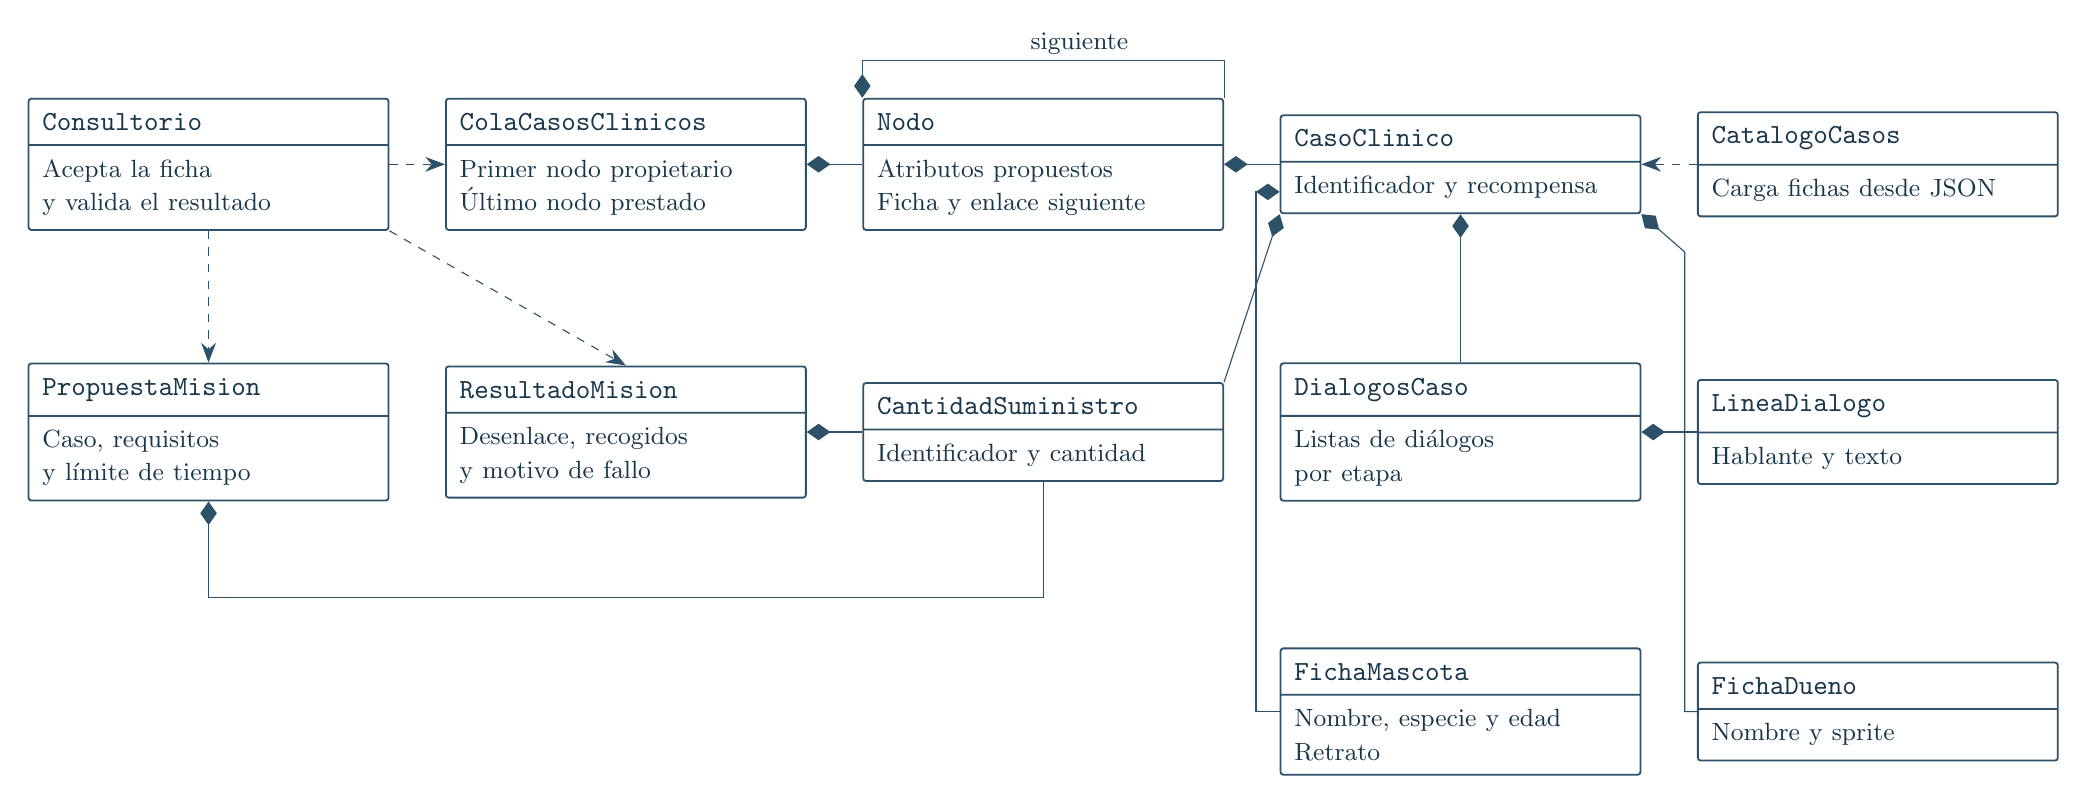
\begin{tikzpicture}
  \clase{consulta}{2.4,10.5}{Consultorio}{Acepta la ficha\\y valida el resultado}
  \clase{cola}{7.7,10.5}{ColaCasosClinicos}{Primer nodo propietario\\Último nodo prestado}
  \clase{nodo}{13,10.5}{Nodo}{Atributos propuestos\\Ficha y enlace siguiente}
  \clase{ficha}{18.3,10.5}{CasoClinico}{Identificador y recompensa}
  \clase{catalogo}{23.6,10.5}{CatalogoCasos}{Carga fichas desde JSON}
  \clase{propuesta}{2.4,7.1}{PropuestaMision}{Caso, requisitos\\y límite de tiempo}
  \clase{resultado}{7.7,7.1}{ResultadoMision}{Desenlace, recogidos\\y motivo de fallo}
  \clase{suministro}{13,7.1}{CantidadSuministro}{Identificador y cantidad}
  \clase{dialogos}{18.3,7.1}{DialogosCaso}{Listas de diálogos\\por etapa}
  \clase{linea}{23.6,7.1}{LineaDialogo}{Hablante y texto}
  \clase{mascota}{18.3,3.55}{FichaMascota}{Nombre, especie y edad\\Retrato}
  \clase{dueno}{23.6,3.55}{FichaDueno}{Nombre y sprite}

  \draw[depende] (consulta) -- (cola);
  \draw[depende] (consulta) -- (propuesta);
  \draw[depende] (consulta.south east) -- (resultado.north);
  \draw[compone] (cola) -- (nodo);
  \draw[compone] (nodo) -- (ficha);
  \draw[compone] (nodo.north west) -- ++(0,.47) -|
    node[etiqueta,pos=.3,above] {siguiente} (nodo.north east);
  \draw[depende] (catalogo) -- (ficha);
  \draw[compone] (ficha.south west) -- (suministro.north east);
  \draw[compone] (ficha) -- (dialogos);
  \draw[compone] (dialogos) -- (linea);
  \draw[compone] ($(ficha.west)+(0,-.35)$) -- ++(-.3,0) |- (mascota.west);
  \draw[compone] (ficha.south east) -- ++(.55,-.48) |- (dueno.west);
  \draw[compone] (resultado) -- (suministro);
  \draw[compone] (propuesta.south) -- ++(0,-1.22) -| (suministro.south);
\end{tikzpicture}

\vfill
\raggedright
Cada ficha requiere uno o más tipos de suministro. Un resultado puede contener
cero o más. El rombo lleno señala qué objeto posee el dato.
La cola posee el primer nodo y cada nodo posee el siguiente, cuando existe.
La definición del tipo interno \texttt{Nodo} y las operaciones quedan a cargo del equipo.

\newpage
\titulo{Veterinaria 2D · Combate, herencia y sprites}
  {Fábrica de enemigos, estrategias y estado que usa la vista}

\centering
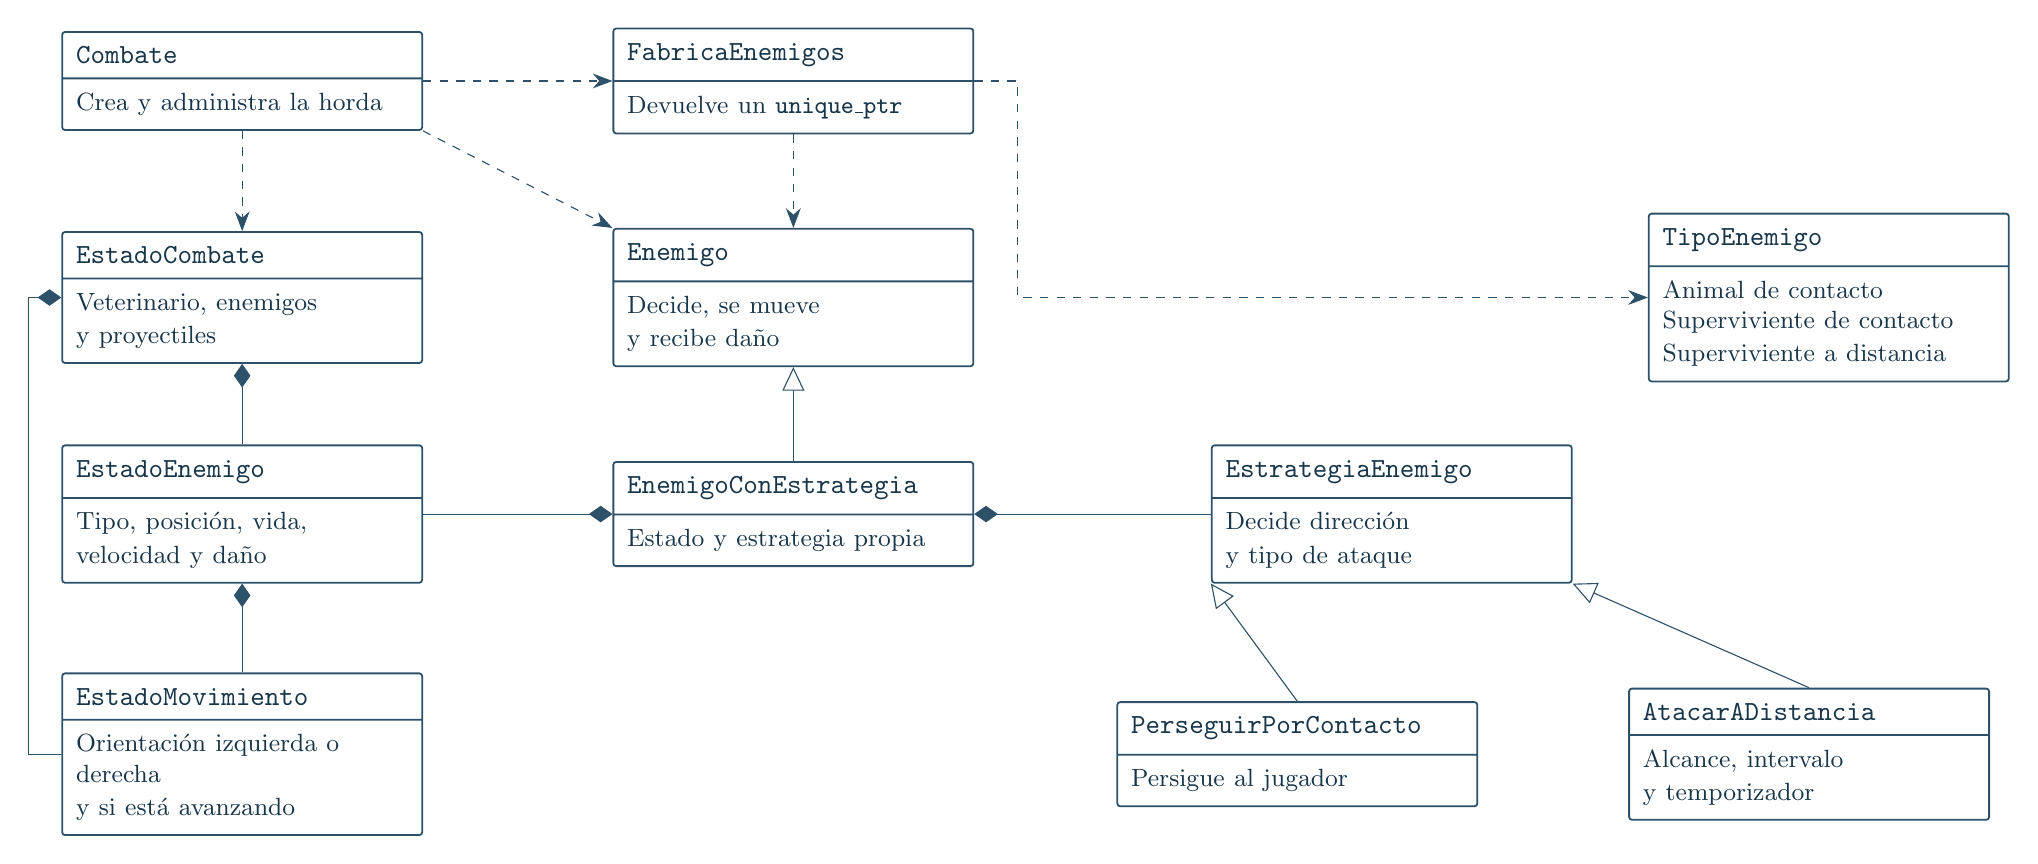
\begin{tikzpicture}
  \clase{combate}{3,10.55}{Combate}{Crea y administra la horda}
  \clase{fabrica}{10,10.55}{FabricaEnemigos}{Devuelve un \texttt{unique\_ptr}}
  \clase{tipo}{23.15,7.8}{TipoEnemigo}{Animal de contacto\\Superviviente de contacto\\Superviviente a distancia}
  \clase{enemigo}{10,7.8}{Enemigo}{Decide, se mueve\\y recibe daño}
  \clase{conestrategia}{10,5.05}{EnemigoConEstrategia}{Estado y estrategia propia}
  \clase{estrategia}{17.6,5.05}{EstrategiaEnemigo}{Decide dirección\\y tipo de ataque}
  \clase{contacto}{16.4,2}{PerseguirPorContacto}{Persigue al jugador}
  \clase{distancia}{22.9,2}{AtacarADistancia}{Alcance, intervalo\\y temporizador}
  \clase{estadoc}{3,7.8}{EstadoCombate}{Veterinario, enemigos\\y proyectiles}
  \clase{estadoe}{3,5.05}{EstadoEnemigo}{Tipo, posición, vida,\\velocidad y daño}
  \clase{mov}{3,2}{EstadoMovimiento}{Orientación izquierda o derecha\\y si está avanzando}

  \draw[depende] (combate) -- (fabrica);
  \draw[depende] (combate.south east) -- (enemigo.north west);
  \draw[depende] (fabrica) -- (enemigo);
  \draw[depende] (fabrica.east) -- ++(.55,0) |- (tipo.west);
  \draw[hereda] (conestrategia) -- (enemigo);
  \draw[compone] (conestrategia) -- (estrategia);
  \draw[hereda] (contacto.north) -- (estrategia.south west);
  \draw[hereda] (distancia.north) -- (estrategia.south east);
  \draw[depende] (combate) -- (estadoc);
  \draw[compone] (estadoc) -- (estadoe);
  \draw[compone] (conestrategia) -- (estadoe);
  \draw[compone] (estadoe) -- (mov);
  \draw[compone] (estadoc.west) -- ++(-.42,0) |- (mov.west);
\end{tikzpicture}

\vfill
\raggedright
El triángulo vacío apunta a la clase base. La fábrica selecciona la estrategia
según el tipo de aparición. Los animales y algunos supervivientes atacan por
contacto. Otros supervivientes atacan a distancia. La vista selecciona los
sprites según el tipo, la orientación y el movimiento.

\newpage
\titulo{Veterinaria 2D · Mascotas y armas}
  {Jerarquías previstas para extender las especies y las armas}

\centering
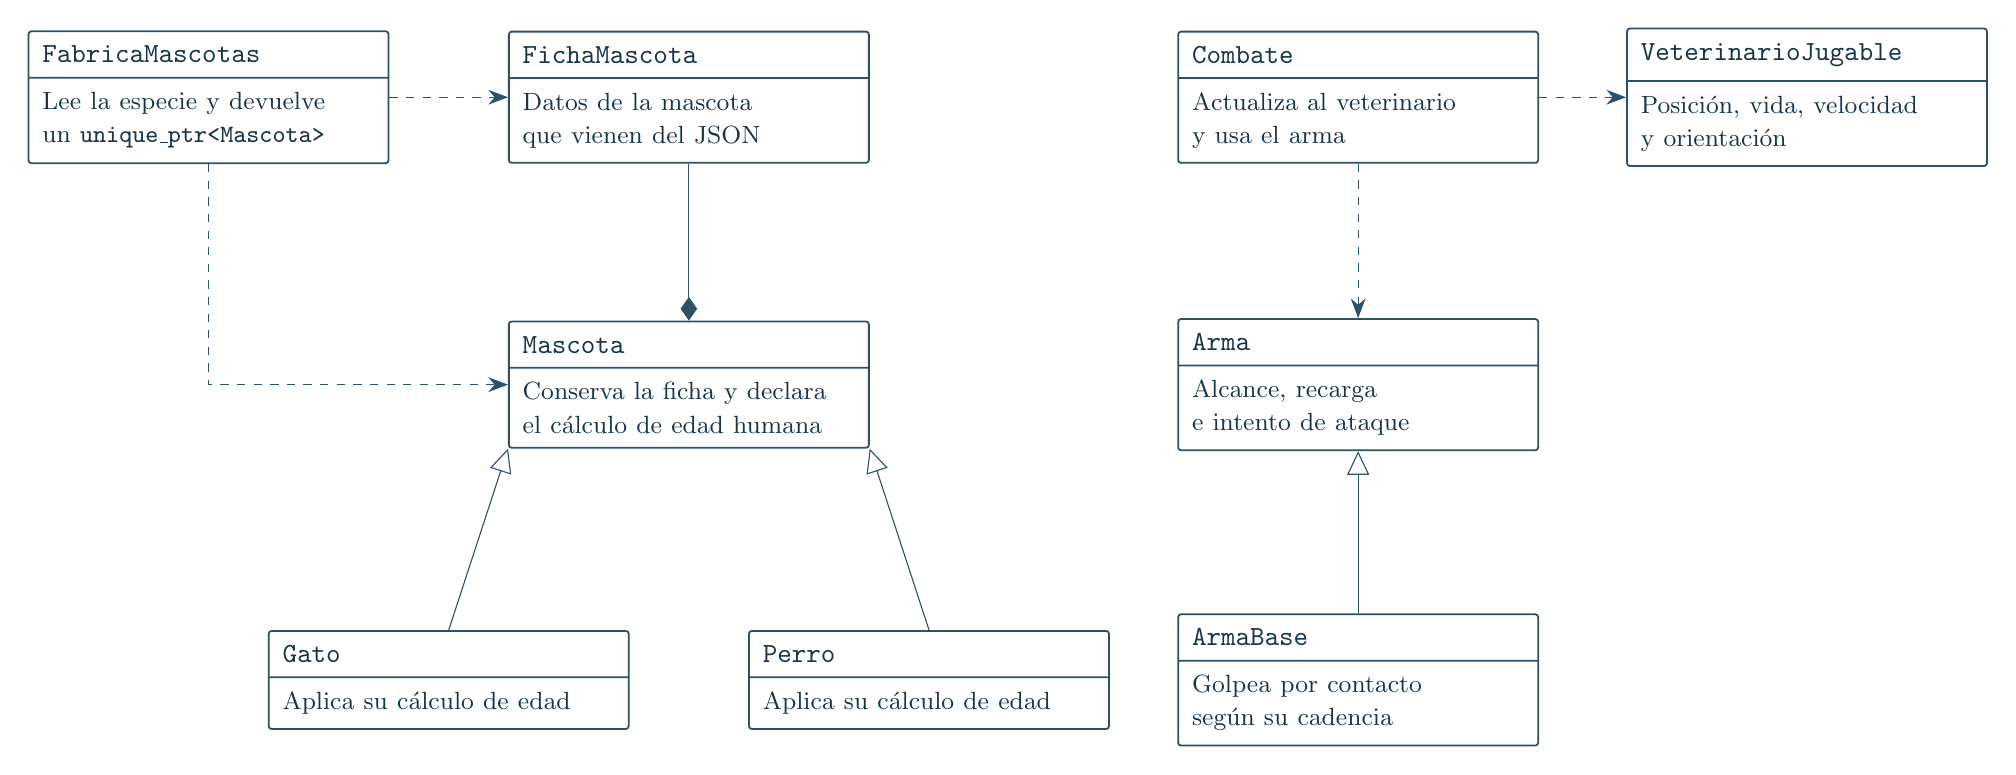
\begin{tikzpicture}
  \clase{fabrica}{3.2,9.9}{FabricaMascotas}{Lee la especie y devuelve\\un \texttt{unique\_ptr<Mascota>}}
  \clase{ficha}{9.3,9.9}{FichaMascota}{Datos de la mascota\\que vienen del JSON}
  \clase{mascota}{9.3,6.25}{Mascota}{Conserva la ficha y declara\\el cálculo de edad humana}
  \clase{gato}{6.25,2.5}{Gato}{Aplica su cálculo de edad}
  \clase{perro}{12.35,2.5}{Perro}{Aplica su cálculo de edad}
  \clase{veterinario}{23.5,9.9}{VeterinarioJugable}{Posición, vida, velocidad\\y orientación}
  \clase{combate}{17.8,9.9}{Combate}{Actualiza al veterinario\\y usa el arma}
  \clase{arma}{17.8,6.25}{Arma}{Alcance, recarga\\e intento de ataque}
  \clase{base}{17.8,2.5}{ArmaBase}{Golpea por contacto\\según su cadencia}

  \draw[depende] (fabrica) -- (ficha);
  \draw[depende] (fabrica.south) |- (mascota.west);
  \draw[compone] (mascota) -- (ficha);
  \draw[hereda] (gato.north) -- (mascota.south west);
  \draw[hereda] (perro.north) -- (mascota.south east);
  \draw[depende] (combate) -- (veterinario);
  \draw[depende] (combate) -- (arma);
  \draw[hereda] (base) -- (arma);
\end{tikzpicture}

\vfill
\raggedright
Agregar otro gato o perro requiere una ficha nueva. Si se añade otro comportamiento,
el equipo implementa una subclase. Combate resuelve el contacto y el arma
determina cuándo puede aplicar daño.
\end{document}
